\subsection{General Overview} \label{arch:general Overview}
In this section, we look at the architecture of MedChain system. We first begin by considering the requirements that our software solution should be able to fulfil. Then, we discuss how our solution satisfies the requirements and objectives. 

% Full discussion of MedChain architecture design requirements, its final architecture, and the reasoning behind certain choices made in the design. Trying to make it as visual as possible with quality figures. 

% \textbf{Question}: Is it necessary that I contrast the work that has been done last semester and this semester \textit{in this section} as well?? If yes,  any ideas how I can best do that?


\subsection{Requirements} \label{arch:requirements}

The main goal of MedChain is to offer distributed access management mechanisms for MedCo. We started to design and implement MedChain last semester in another project. The main goal of this project is to improve MedChain software already implemented, develop a docker-based implementation of MedChain and integrate MedChain into MedCo described in Section \ref{background:medco}. To achieve this, Medchain has to fulfil the following tasks and requirements:
% \begin{enumerate}
%     \item Offer its services in a distributed manner 
%     \item Offer access management and user authentication 
%     \item Authorize users and queries
%     \item Enable auditability by recording a full history of queries in blockchain
%     \item Work seamlessly with MedCo
% \end{enumerate}
% In the following sections, we study how each of the above-mentioned requirements are fulfilled in Medchain. 

% \subsubsection{Distributed Services in Medchain} \label{arch:distributed}
% As it was mentioned in the previous section, the first goal of Medchain is to offer services in a distributed manner. To achieve this, we used conodes. Conodes make the foundation for Medchain. They support distributed protocols and services provided by the \href{https://github.com/dedis/onet/blob/master/README.md}{onet} library (a part of Cothority project developed by DEDIS at EPFL). Consequently, Medchain is able to offer access management in a distributed manner. 

% \subsubsection{Authentication in Medchain}\label{arch:authentication}
% The goal of authentication is to verify the identity of the user who wants to access a specific resource such as data. In Medchain, user authentication is delegated to Keycloak \cite{keycloak:2019} which is the identity provider. This means that once Medchain receives a query from a user, we can simply assume that he/she is already authenticated and his/her identity and the user identity is submitted to Medchain as part of the query. We will discuss this in more details in Section \ref{arch:flow}, where the flow of query in Medchain is described comprehensively.

\subsubsection{Authorization in Medchain}\label{arch:authorization}
The goal of authorization is to control the user access to resources (e.g., sensitive medical data) based on agreed rules. In MedChain, we use Darcs (described in Section \ref{background:darc}) to enable user authorization and access management. 


\subsubsection{Distributed Immutable Logging in MedChain} \label{arch:audit}
% Auditability in Medchain means that there should be a mechanism in place so that the users can track all the queries submitted to Medchain server. Consequently, trace of any data misuse, data abuse, security/privacy breach, etc. can be found and mitigated later. 

In MedChain, we use blockchains to offer distributed auditability. The blockchain framework we use in MedChain is ByzCoin (see Section \ref{background:byzcoin}). Every query sent to MedCo by the user as well as its status, whether it is authorized or rejected, is recorded in the immutable ledger that is accessible at every MedChain node in the network.  

\subsection{Medchain High-level View} \label{arch:high-level view}

Figure \ref{fig:medchain_node} shows how a MedChain node looks like. Every MedChain node is a customized Conode (see section \ref{section4} for further details) and has one or more projects defined in it. Projects specify user access controls and define data resources. Each project contains three important building blocks. Below you can find more about projects and their building blocks:
\begin{itemize}
    \item \textbf{Projects}: specify rules for users to access data resources using access right controls.
    \item \textbf{Smart contracts}: define data, in this case key-value pairs of the query (i.e., the key) and its status (i.e., the value), that is stored in distributed ledger
    \item \textbf{Darcs}: define and manage user's access to resources. Every project is attached to a single Darc that determines user access rules for the database governed by the project. 
    \item \textbf{Blockchain}: system audit. It is possible to retrieve a record of all queries submitted to MedChain for authorization to check the content of query and the querier's identity. 
\end{itemize}


\begin{figure}[ht] 
        \centering 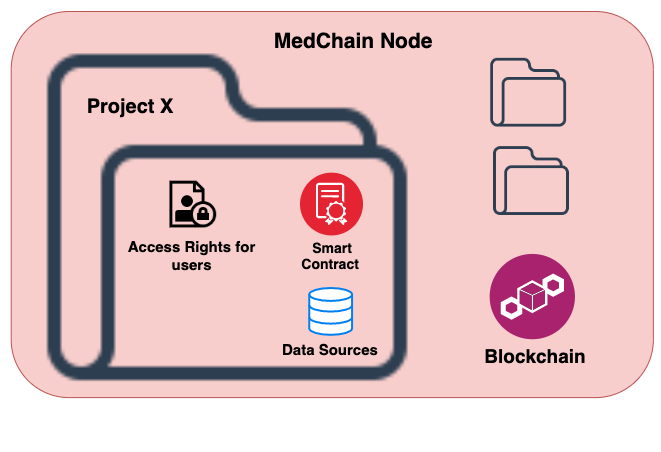
\includegraphics[width=0.7\columnwidth]{Images/medchain_node.png}
        \caption{\label{fig:medchain_node} 
         The structure and building blocks of a MedChain node.
        }
\end{figure}




\subsection{Flow of Queries in Medchain}\label{arch:flow}

Figure \ref{fig:medchain_workflow} illustrates the full architecture of MedChain and its detailed workflow starting from query creation and submission by the client until the query is executed. The numbers used in the figure correspond to the steps described below. Also, parts outlined with dashed-line represent the contributions done in this project (further explained in Sections \ref{section4}, \ref{section5}, and \ref{section6}).

% In this figure, there are three hospitals each running their own local Medchain server (conode). Now, focusing only on the user at Hospital 1, we describe the enumerated steps in Figure \ref{fig:medchain_workflow} as following:

\begin{enumerate}
    \item \textbf{User Login}: Client receives the token (i.e., its identity) from Keycloak (using OpenID Connect).
    
    \item \textbf{Query Creation \& Submission}: User spawns a query. The query is submitted to MedCo-connector (i.e., query orchestrator). Figure \ref{fig:medco_query} shows the simplified structure of a MedCo-connector (explore) query. 
  \begin{figure}[htbp] 
        \centering 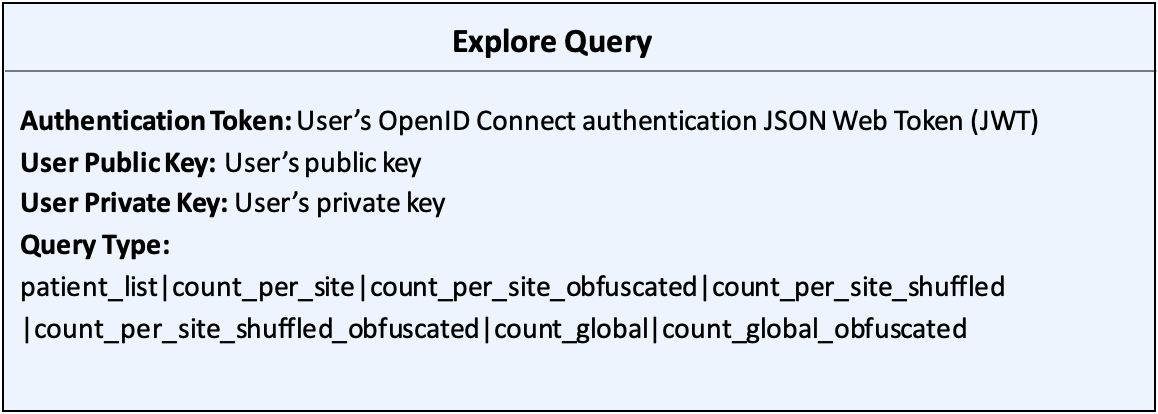
\includegraphics[width=0.9\columnwidth]{Images/medco_query.png}
        \caption{\label{fig:medco_query} 
         Simplified structure of a MedCo-connector (explore) query.
        }
\end{figure}
    
    \item \textbf{User Authentication}: MedCo-connector verifies the token (i.e., the identity) of the user and authenticates it. 
    
    \item \textbf{Submission of Query To Medchain}: MedCo-connector receives the user identity and user query. It then sends the query that contains the user’s identity (i.e., part of the token) to MedChain server for authorization. The query that MedChain receives is a key-value pair data structure shown in Figure \ref{fig:medchain_query}:
\begin{figure}[htbp] 
        \centering 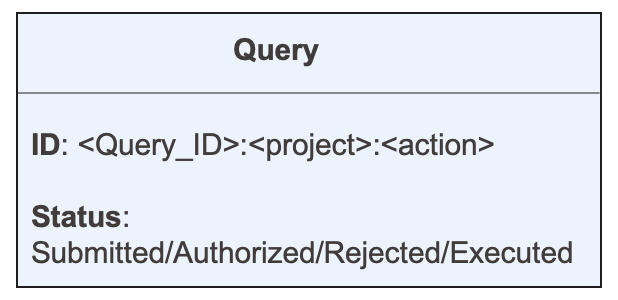
\includegraphics[width=0.5\columnwidth]{Images/query.png}
        \caption{\label{fig:medchain_query} 
         MedChain query data structure
        }
\end{figure}

%     \begin{verbatim}
%         {ID:<Query ID>,Status:<Query Status>}
%     \end{verbatim}
% The query itself has the following format:
%   \begin{verbatim}
%       <user_id>:<databaseX>:<type of query>
%   \end{verbatim}
  Where \texttt{<Query\_id>} contains part of the user's token provided by Keycloak, \texttt{<project>} is the name of the project (i.e., the database) the user is querying, and \texttt{<action>} is what the user is trying to access from the database which can be one of the below:
  \begin{itemize}
        \item \texttt{patient\_list}
        \item \texttt{count\_per\_site}
        \item \texttt{count\_per\_site\_obfuscated}
        \item \texttt{count\_per\_site\_shuffled}
        \item \texttt{count\_per\_site\_shuffled\_obfuscated}
        \item \texttt{count\_global}
        \item \texttt{count\_global\_obfuscated}
  \end{itemize}
   
  Finally, \texttt{Status} is the status of the query in MedChain and it could be: \texttt{"Submitted"}, \texttt{"Authorized"}, \texttt{"Rejected"}, or \texttt{"Executed"} .

    \item \textbf{Query Transaction Creation}: \label{workflow:step 5}
    MedChain retrieves the ID o the Darc based on the name of the project and creates a normal (i.e., not deferred, see later) transaction to spawn a \texttt{Query} (i.e., an instance of \texttt{MedChain Contract}) and signs it. The transaction looks like below:
        \begin{verbatim}
CreateTransaction(byzcoin.Instruction{
    InstanceID:    byzcoin.NewInstanceID(<Project X Darc ID>),
    Spawn: &byzcoin.Spawn{
        ContractID: MedChainContractID,
        Args: byzcoin.Arguments{
                {
                    Name:  <Query_id>:<projectX>:<action>,
                    Value: []byte("Submitted"),
                },
        },
})
        \end{verbatim}
        
    \item \textbf{Query Authorization}: MedChain retrieves the Darc governing the instance and checks the user authorizations for the \texttt{<action>}. Depending on the result of authorization checks one of the below scenarios happens:
    \begin{itemize}
        \item If the Darc rules \textbf{are not met} (i.e., user is not allowed to query \texttt{<action>}), the query is immediately rejected. Consequently, a new transaction is created by MedChain that \textit{updates} query \texttt{Status} to \texttt{Rejected} and adds the transaction to the ledger. Also, a message containing the new query status is sent back to MedCo-connector in order to notify it of authorization rejection (this is more explained in Section \ref{section4} where MedChain API calls are described)
        
        \item If the Darc rules \textbf{are met}, the query is authorized. Hence, two new transactions are created by MedChain. The first one is a normal transaction that updates the query \texttt{Status} to \texttt{Authorized} which is only signed by this MedChain node and is immediately written to the ledger. The second transaction, however, is a \textit{deferred} transaction (see Section \ref{section4}). By spawning a deferred transaction, MedChain node proposes a transaction to the whole MedChain network i.e., it broadcasts the instance ID of deferred transaction to rest of the MedChain nodes in network. Then, users at other MedChain nodes need to \textit{sign} the transaction using the instance ID they receive. When the rules of Darc are met (i.e., a threshold number of signatures are added to the proposed transaction), the transaction can be executed by any of the signers (only one execution is allowed for every proposed transaction). It is important to note that even if all users can sign the transaction, it can only be executed once the rules of corresponding Darc are met. 
        Once the proposed transaction is successfully executed, the transaction is added to the ledger and MedChain sends MedCo-connector a message containing the status of query as \texttt{Authorized}.  
    \end{itemize}
     
    \item \textbf{Query Authorization Result}: In the mean time, MedCo-connector is waiting for a reply from MedChain node. Once authorization (step 6) is done, MedChain sends the result (i.e., query status) back to MedCo-connector which is either \texttt{Authorized} or \texttt{Rejected}. 
    
    \item \textbf{Query Execution and Committing Final Query Status To The Ledger}: If MedCo-connector learns that the query has been rejected through a message from MedChain node, it will not execute the query. Otherwise, MedCo-connector executes the query and once done, sends a message back to MedChain so that the status of query is updated to \texttt{Executed} and is written to the ledger.

\end{enumerate}
 
 
 The explained workflow and its mechanisms such as MedChain to MedChain communications (i.e., message propagation among MedChain nodes) and API calls have been fully implemented in this project. 
 
 \begin{figure}[htbp] 
        \centering 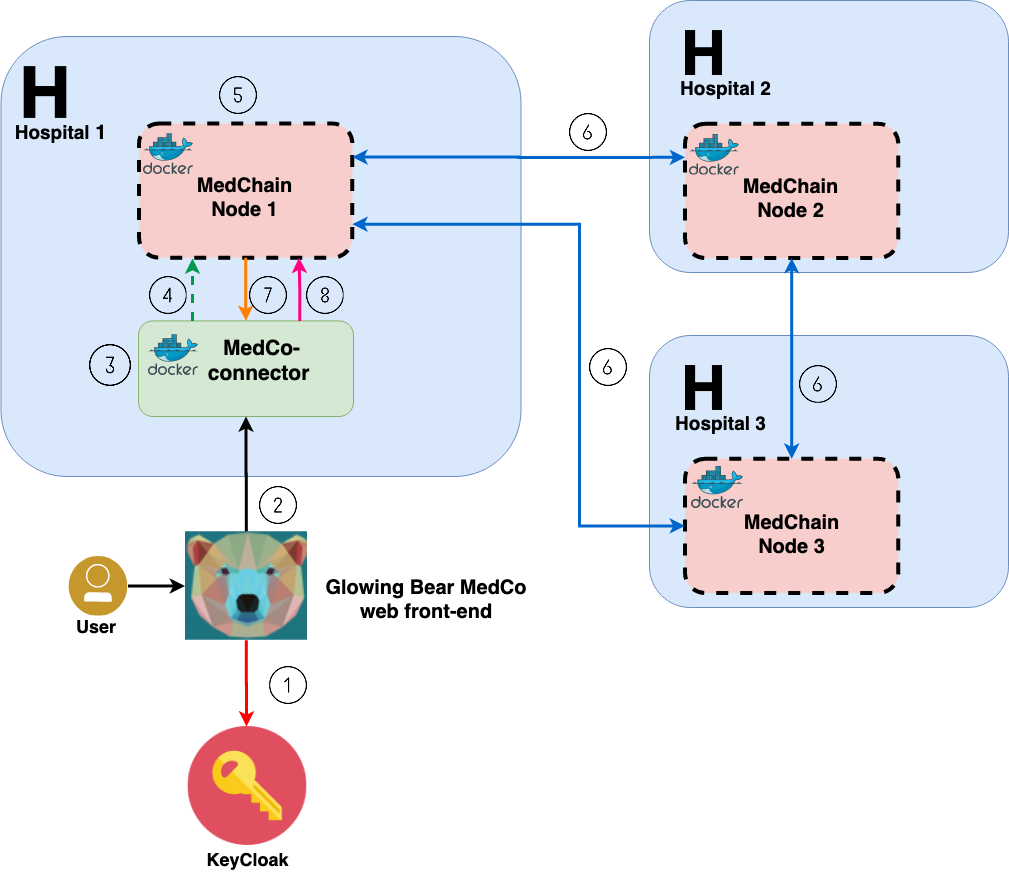
\includegraphics[width=1\columnwidth]{Images/arch-updated.png}
        \caption{\label{fig:medchain_workflow} 
         Medchain architecture: workflow of queries in MedChain.
        }
\end{figure}
